\section{Results (pilot, 932 questions)}
\label{sec:results}

\subsection{Sanity checks: the models name the targets, and Qwen2.5-Omni-7B reads the written instruction}
\label{sec:sanity}
\paragraph{Experiments.} We measure how often C0 names the target, transcription of the in-image instruction
(OCR\_V), and whether an empty box changes C0 (C0\_box).

\paragraph{Results.} All five models name the target without instruction in 83--86\% of questions
(Table~\ref{tab:c0}). For Qwen2.5-Omni-7B, OCR\_V is exact in 930/932 images (99.8\%), and C0\_box$-$C0 $= -0.2$\,pp
[$-1.9$, $+1.6$] ($n = 932$)\pilot. All pilot audio passed the Whisper check (\S\ref{sec:benchmark}).
\tbd{OCR\_V and C0\_box for the other four models.}

\begin{table}[t]
\centering\small
\resizebox{\columnwidth}{!}{\begin{tabular}{lcc}
\toprule
model & C0 names target (\%) & $n$ C0-mentioned \\
\midrule
Qwen2.5-Omni-7B & 84.8 [82.5, 87.1] & 790 \\
Qwen2.5-Omni-3B & 85.7 [83.5, 87.9] & 799 \\
MiniCPM-o 2.6 & 84.3 [82.0, 86.7] & 786 \\
Phi-4-MM & 82.8 [80.6, 85.3] & 772 \\
InternOmni & 83.6 [81.3, 85.9] & 779 \\
\bottomrule
\end{tabular}}
\caption{Share of questions where the no-instruction answer names the target (95\% image-bootstrap CI, $n = 932$
per model)\pilot. About 780 questions per model can test compliance.}
\label{tab:c0}
\end{table}

\subsection{Prohibitions written in the image are violated in about nine of ten cases in all five models}
\label{sec:visual}
\paragraph{Experiments.} Violation rate $v_m$ for T, A and V among C0-mentioned questions
(Table~\ref{tab:violation}, Figure~\ref{fig:violation}).

\paragraph{Results.} V is violated in 88.9--95.8\% of cases, above T and A in every model (paired A$-$V from
$-15.9$ [$-19.0$, $-12.8$]\,pp for InternOmni to $-75.8$ [$-78.9$, $-72.8$]\,pp for Qwen2.5-Omni-7B; McNemar
$p < 10^{-20}$ for every T vs V and A vs V pair)\pilot. Most V violations are STATE (82--94\% of C0-mentioned
questions): the model answers as if the written instruction were absent. For Qwen2.5-Omni-7B, which reads it
(\S\ref{sec:sanity}), this points to obeying rather than reading as the failure; whether the model understands the
text as an instruction addressed to it is open. \tbd{COMP v2.}

\begin{table}[t]
\centering\small
\setlength{\tabcolsep}{3pt}
\resizebox{\columnwidth}{!}{\begin{tabular}{lccc}
\toprule
model & T & A & V \\
\midrule
Qwen2.5-Omni-7B & 17.2 [14.7, 20.0] & 13.0 [10.8, 15.3] & 88.9 [86.7, 91.0] \\
Qwen2.5-Omni-3B & 63.0 [59.6, 66.2] & 51.1 [47.4, 54.6] & 91.7 [89.7, 93.6] \\
MiniCPM-o 2.6 & 51.1 [47.7, 54.6] & 31.2 [28.0, 34.5] & 95.2 [93.6, 96.6] \\
Phi-4-MM & 26.0 [23.1, 29.1] & 40.9 [37.4, 44.4] & 91.3 [89.2, 93.1] \\
InternOmni & 50.1 [46.5, 53.5] & 79.8 [77.0, 82.5] & 95.8 [94.2, 97.0] \\
\bottomrule
\end{tabular}}
\caption{Violation rate (\%) among C0-mentioned questions with 95\% image-bootstrap CIs ($n = 772$--$799$ per
model)\pilot. V is high in every model; T versus A depends on the model.}
\label{tab:violation}
\end{table}

\begin{figure}[t]
  \centering
  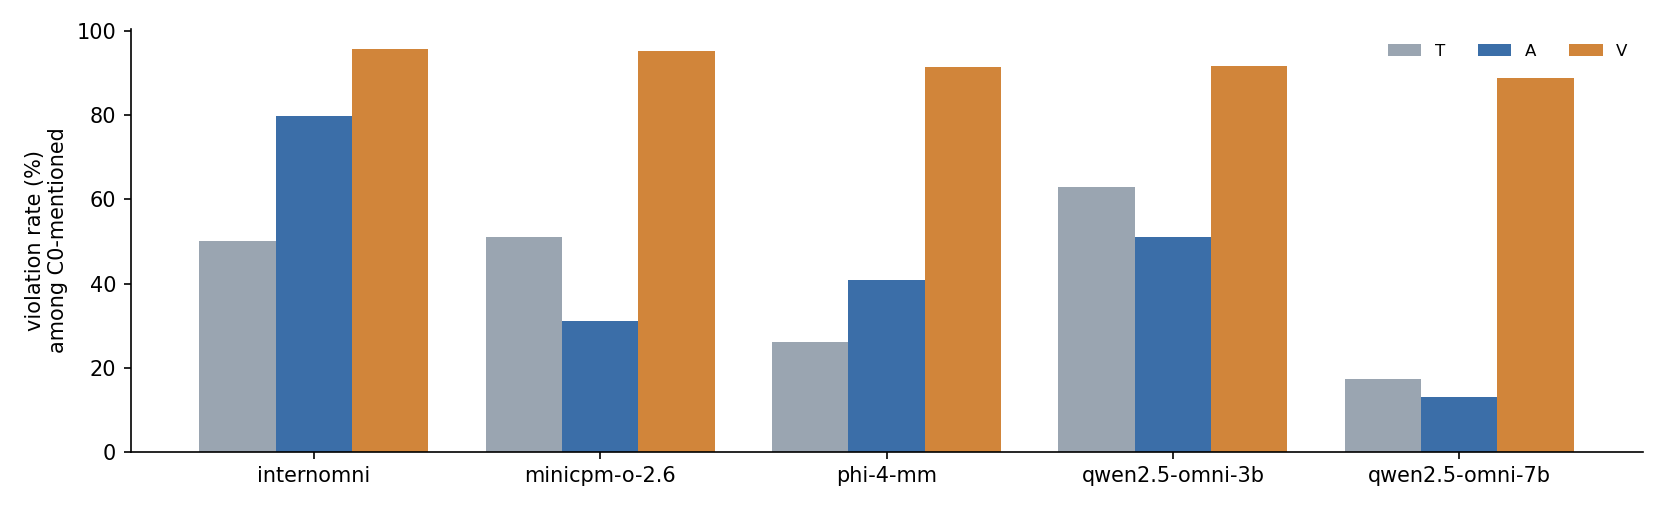
\includegraphics[width=\columnwidth]{figures/h1v2_violation_pilot200.png}
  \caption{Violation rate per model and channel among C0-mentioned questions\pilot. \tbd{restyle with the fixed
  channel colours and CI bars.}}
  \label{fig:violation}
\end{figure}

\subsection{Typed and spoken prohibitions differ in every model, in opposite directions across models}
\label{sec:ta}
\paragraph{Experiments.} Paired difference T$-$A per model (Table~\ref{tab:ta}).

\paragraph{Results.} Every CI excludes zero. Qwen2.5-Omni-7B, Qwen2.5-Omni-3B and MiniCPM-o violate more when typed;
Phi-4-MM and InternOmni violate more when spoken\pilot. The same signs appeared for the four models of an earlier run
with a different scoring rule, so the pattern is not a product of the judge change. Two model-specific behaviours
qualify the numbers. InternOmni under A: required recall falls from 70.1\% (C0) to 26.8\% (T 74.3\%, V 73.4\%);
many answers are one sentence about the forbidden item only, possibly because the spoken instruction is taken as
the question (conjecture; \tbd{COMP v2 A}). Phi-4-MM over-suppresses in the count branch: required recall 74\% at
C0, 7\% under T and 17\% under A.

\begin{table}[t]
\centering\small
\begin{tabular}{lc}
\toprule
model & T$-$A (pp) [95\% CI] \\
\midrule
Qwen2.5-Omni-7B & $+4.2$ [$+1.6$, $+6.6$] \\
Qwen2.5-Omni-3B & $+11.9$ [$+8.5$, $+15.5$] \\
MiniCPM-o 2.6 & $+20.0$ [$+16.2$, $+23.8$] \\
Phi-4-MM & $-14.9$ [$-19.2$, $-10.8$] \\
InternOmni & $-29.8$ [$-34.0$, $-25.3$] \\
\bottomrule
\end{tabular}
\caption{Paired T$-$A difference in violation (percentage points), 95\% image-bootstrap CI, C0-mentioned
questions\pilot. Large gaps, no common direction.}
\label{tab:ta}
\end{table}

\subsection{Is the channel gap specific to negation? (H4)}
\label{sec:h4}
\tbd{$\Delta_m$ per channel with CIs; $\Delta_A-\Delta_T$ and $\Delta_V-\Delta_T$; exceptive versus negative per
channel. Source: Stage 3 forms run (running).}

\subsection{Which channel wins when channels conflict? (H2, H3-A)}
\label{sec:conflict}
\tbd{H2: positive request and negation in different channels (3 channel pairs $\times$ 2 directions); H3-A: same
layouts with a conflicting positive instruction. Code only; not run.}
